\documentclass[fontsize=11pt, twoside=off]{scrbook} 
% Dokumentenklasse: KOMA-Script Book

\usepackage[utf8]{inputenc}
\usepackage[T1]{fontenc} % Zeichensatzkodierung

\usepackage{calc} % Berechnungen
\usepackage[english]{babel} % Deutsche Lokalisierung
\usepackage{graphicx} % Grafiken
\usepackage[export]{adjustbox}
\usepackage[absolute, overlay]{textpos} % Positionierung
\usepackage{bbm}

%\usepackage{paralist}
\usepackage[linesnumbered]{algorithm2e}
\usepackage{amsmath}
\usepackage{colortbl}
%\usepackage{bbold}
\usepackage[hang,small]{subfigure} 
\usepackage{graphicx}
\usepackage[style=numeric-comp,autocite=superscript,backend=bibtex]{biblatex}
\setbeamertemplate{bibliography item}{}
\usepackage{lipsum}

% Silbentrennung:
\usepackage{hyphenat}
%\tolerance 2414
%\hbadness 2414
%\emergencystretch 1.5em
%\hfuzz 0.3pt
%\widowpenalty=10000     % Hurenkinder
%\clubpenalty=10000      % Schusterjungen
%\vfuzz \hfuzz

% Euro-Symbol:
\usepackage[gen]{eurosym}
\DeclareUnicodeCharacter{20AC}{\euro{}}

% Schriftart Helvetica:
%\useinnertheme{default}
%\usefonttheme{professionalfonts}
%\usefonttheme{serif}
%\renewcommand\mathfamilydefault{\rmdefault}
\usefonttheme[onlymath]{serif}
\renewcommand\sfdefault{cmbr}

\usepackage[scaled]{helvet}
\renewcommand{\familydefault}{\sfdefault}
%\usepackage{mathptmx} % skalierbare Formelschriften
\usepackage{tabularx}
\usepackage{multicol} % mehrspaltiger Text
\usepackage{tikz}
\usetikzlibrary{arrows, shapes, shapes.multipart, trees, positioning,
    backgrounds, fit, matrix}

% Diagramme:
\usepackage{pgfplots}
\pgfplotsset{compat=default}

% Erweiterbare Fusszeile:
\newcommand{\PraesentationSchriftgroesseSehrGross}{\fontsize{30}{45}}
\newcommand{\PraesentationSchriftgroesseGross}{\fontsize{22}{33}}
\newcommand{\PraesentationSchriftgroesseNormal}{\fontsize{16}{29}}
\newcommand{\PraesentationSchriftgroesseKlein}{\fontsize{12}{18}}
\newcommand{\PraesentationSchriftgroesseDreizeiler}{\fontsize{7}{10}}
\newcommand{\PraesentationSchriftgroesseAufzaehlungszeichen}{\fontsize{10}{15}}
\newcommand{\PraesentationAbstandAbsatz}{22.1pt}
\newcommand{\PraesentationPositionKorrekturOben}{-0.75cm}
\newcommand{\PraesentationBeispieleSchriftgroessen}{30 | 22 | 16 | 12}

    % Blautöne:
\definecolor{TUMBlau}{RGB}{0,101,189} % Pantone 300
\definecolor{TUMBlauDunkel}{RGB}{0,82,147} % Pantone 301
\definecolor{TUMBlauHell}{RGB}{152,198,234} % Pantone 283
\definecolor{TUMBlauMittel}{RGB}{100,160,200} % Pantone 542

    % Hervorhebung:
\definecolor{TUMElfenbein}{RGB}{218,215,203} % Pantone 7527 -Elfenbein
\definecolor{TUMGruen}{RGB}{162,173,0} % Pantone 383 - Grün
\definecolor{TUMOrange}{RGB}{227,114,34} % Pantone 158 - Orange
\definecolor{TUMGrau}{gray}{0.6} % Grau 60%


%%%%%%%%%%%%%%%%%%%%%%%%%%%%%%%%%%%%%%%%%%%%%%%%%%%%%%%
% Personenspezifische Informationen
%%%%%%%%%%%%%%%%%%%%%%%%%%%%%%%%%%%%%%%%%%%%%%%%%%%%%%%%
% Für die Person anpassen:
\newcommand{\PersonAdresse}{%
    @Adresse@\\%
    @Plz@~\PersonStadt%
}
\newcommand{\PersonTelefon}{@Telefon@}
\newcommand{\PersonFax}{@Fax@}
\newcommand{\PersonEmail}{@E-Mail@}
\newcommand{\PersonWebseite}{@Web@}

\newcommand{\FakultaetAnsprechpartner}{@Ansprechpartner@}
% Fakultät:
\newcommand{\EinstellungBankName}{Bayerische Landesbank}
\newcommand{\EinstellungBankIBAN}{DE10700500000000024866}
\newcommand{\EinstellungBankBIC}{BYLADEMM}
\newcommand{\EinstellungSteuernummer}{143/241/80037}
\newcommand{\EinstellungUmsatzsteuerIdentifikationsnummer}{DE811193231}

\hyphenation{} % eigene Silbentrennung

\newcommand{\suchthat}{\;\ifnum\currentgrouptype=16 \middle\fi|\;}
\newcommand{\norm}[1]{\left\Vert#1\right\Vert}
\newcommand{\abs}[1]{\left\vert#1\right\vert}
\newcommand{\iprod}[1]{\left\langle#1\right\rangle}
\newcommand{\eps}{\varepsilon}
\newcommand{\BibLaTeX}{{Bib}\LaTeX~}
\newcommand{\memoir}{\text{Memoir}~}
\newcommand{\dd}{\mathrm{d}}
\newcommand{\Ex}{\mathop{{}\mathbb{E}}}%\mathop{{}\mathbb{E}}
\newcommand{\I}{\pmb{\mathbb{I}}}%\mathop{{}\mathbb{E}}
\newcommand{\II}[2]{{\mathbbm{I}_{#1}\left[#2\right]}}
\newcommand{\cov}{\mathrm{Cov}}
\newcommand{\var}{\mathrm{Var}}
\newcommand{\deter}{\mathrm{det}}
\newcommand{\tran}{\mathsf{T}}
\newcommand{\matlab}{$\text{MATLAB}^{\text{\textregistered}}$~}
\newcommand{\defin}{\textit}
\newcommand{\intd}{\text{d}}
\newcommand{\N}{\mathrm{N}}
\newcommand{\logN}{\mathrm{logN}}
\newcommand{\diver}{\mathrm{div}}
\newcommand{\ve}[1]{{\boldsymbol{#1}}}
\DeclareMathOperator{\argmin}{argmin}
\DeclareMathOperator{\ble}{BLE}
\DeclareMathOperator{\enkfip}{EnKF}
\DeclareMathOperator{\E}{\mathbb{E}}
\DeclareMathOperator{\Cov}{Cov}
\DeclareMathOperator{\Var}{Var}
\DeclareMathOperator{\iid}{i.i.d.}
\newcommand{\highlight}[1]{\colorbox{TUMBlauHell}{$\displaystyle #1$}}
 % !!! NICHT ENTFERNEN !!!
%%%%%%%%%%%%%%%%%%%%%%%%%%%%%%%%%%%%%%%%%%%%%%%%%%%%%%%%%%%%%%%%%%%%%%%%%%%%%%%%
% EINSTELLUNGEN
%%%%%%%%%%%%%%%%%%%%%%%%%%%%%%%%%%%%%%%%%%%%%%%%%%%%%%%%%%%%%%%%%%%%%%%%%%%%%%%%
\KOMAoptions{parskip=full}

% Seitenränder:
\newcommand{\SeitenrandOben}{25.8mm}
\newcommand{\SeitenrandRechts}{21mm}
\newcommand{\SeitenrandLinks}{35mm}
\newcommand{\SeitenrandUnten}{24.8mm}
\newcommand{\FusszeileHoehe}{11.7mm}

\usepackage[a4paper,
    head=16.5pt,
    top=\SeitenrandOben,
    bottom=\SeitenrandUnten,
    inner=\SeitenrandLinks,
    outer=\SeitenrandRechts
]{geometry}


% Fußzeilen:
\setlength{\footheight}{\FusszeileHoehe}
\clearscrheadfoot
\ifoot*{\Thema\vfill}
\ofoot*{\pagemark\vfill}
\setkomafont{pageheadfoot}{\fontsize{9pt}{13pt}\normalfont}
\setkomafont{pagefoot}{\normalfont}%\bfseries
\setkomafont{pagenumber}{\normalfont}
\pagestyle{scrheadings}


% Fußnoten:
\KOMAoptions{%
    %footnotes=multiple % mehrere Fußnoten werden durch Zeichen getrennt
}
%\setfootnoterule[.6pt]{5.08cm}
\renewcommand{\footnoterule}{\hrule width 5.08cm height .6pt \vspace*{3.9mm}}
%\setlength{\footnotesep}{5mm}
\deffootnote{2mm}{2mm}{%
    \makebox[2mm][l]{\textsuperscript{\thefootnotemark}}%
}
\setkomafont{footnoterule}{\fontsize{9pt}{20pt}\selectfont}


% Überschriften:
\KOMAoptions{%
    open=any, % keine Festlegung auf linke oder rechte Seite
    numbers=noendperiod, % kein automatischer Punkt nach Gliederungsnummer
    headings=small
}

\makeatletter
\g@addto@macro{\@afterheading}{\vspace{-\parskip}} % \parskip nach Gliederungsbefehlen entfernen
\renewcommand*{\chapterheadstartvskip}{\vspace{\@tempskipa}\vspace{-3pt}} % Korrektur für Abstand über Kapitelüberschriften
\makeatother

\setkomafont{disposition}{\normalfont\sffamily}

\setkomafont{chapter}{\bfseries\fontsize{19pt}{22pt}\selectfont}
\RedeclareSectionCommand[%
  beforeskip=0pt,
  afterskip=29pt
]{chapter}
\renewcommand*{\chapterformat}{\thechapter.\enskip} % Immer Punkt nach Kapitelnummer

\setkomafont{section}{\fontsize{15pt}{17pt}\selectfont}
\RedeclareSectionCommand[%
  beforeskip=0pt,
  afterskip=24.1pt
]{section}
\renewcommand*{\sectionformat}{\makebox[13mm][l]{\thesection.\enskip}} % Feste Breite für Abschnittsnummer und immer Punkt danach

\setkomafont{subsection}{\normalfont\fontsize{12pt}{13pt}\selectfont}
\RedeclareSectionCommand[%
  beforeskip=0pt,
  afterskip=1pt
]{subsection}
\renewcommand*{\subsectionformat}{\makebox[13mm][l]{\thesubsection.\enskip}} % Feste Breite für Unterabschnittsnummer und immer Punkt danach


% Listen:
\setlist{%
    labelsep=0mm,
    itemindent=0pt,
    labelindent=0pt,
    align=left,
    parsep=1.5ex
}
\setlist[itemize]{%
    leftmargin=5mm,
    labelwidth=4.9mm
}
\setlist[itemize,1]{%
    before={\vspace{0.25ex}},
    label={\raisebox{.35ex}{\smaller[2]\textbullet}},
    after={\vspace{-\parsep}\vspace{-.25ex}}
}
\setlist[itemize,2]{%
    label={\raisebox{.35ex}{\rule{.58ex}{.58ex}}}
}
\setlist[enumerate]{%
    leftmargin=10mm,
    labelwidth=9.9mm
}
\setlist[enumerate,2]{%
    label={\alph*.}
}

\setlist[description]{%
%    labelindent=!,
    leftmargin=1em,
    labelwidth=!,
    parsep=0mm,
    partopsep=0mm,
    labelsep=1em,
}


% Verzeichnisse:
\KOMAoptions{%
    toc=flat, % keine Einrückungen im Inhaltsverzeichnis
    toc=chapterentrydotfill, % Punkte bis zur Seitennummer bei Kapiteln
    listof=entryprefix, % Präfix für Einträge in Abbildungs- und Tabellenverzeichnis
    listof=nochaptergap, % Kein Abstand für Kapiteleinträge in extra Verzeichnissen
}

\makeatletter
\renewcommand{\@dotsep}{.3} % Abstand der Füllpunkte

% "chapteratlist" für Inhaltsverzeichnis auswerten:
\renewcommand*{\addchaptertocentry}[2]{%
  \iftocfeature{toc}{chapteratlist}{}{%
    \addtocontents{toc}{\protect\vspace{-5pt}}% extra Abstand vor Kapitelüberschriften in Inhaltsverzeichnis entfernen
  }%
  % Originaldefinition aus scrbook.cls:
  \addtocentrydefault{chapter}{#1}{#2}%
  \if@chaptertolists
    \doforeachtocfile{%
      \iftocfeature{\@currext}{chapteratlist}{%
        \addxcontentsline{\@currext}{chapteratlist}[{#1}]{#2}%
      }{}%
    }%
    \@ifundefined{float@addtolists}{}{\scr@float@addtolists@warning}%
  \fi%
}
\makeatother

\AfterTOCHead[toc]{\protect\vspace{.8ex}} % Abstand zwischen Überschrift und Inhaltsverzeichnis
\setuptoc{toc}{noparskipfake} % Angleichung der Abstände nach Inhaltsverzeichnisüberschrift an andere Überschriften
\unsettoc{toc}{chapteratlist} % kein Abstand vor Kapiteleinträgen im Inhaltsverzeichnis, funktioniert nur durch obige Redefinition von \addchaptertocentry

% -- Abbildungs- und Tabellenverzeichnis:

\AfterTOCHead[lof]{\protect\vspace{-.1ex}\doublespacing} % Abstand zwischen Überschrift und Abbildungsverzeichnis, doppelter Zeilenabstand
\setuptoc{lof}{noparskipfake} % Angleichung der Abstände nach Abbildungsverzeichnisüberschrift an andere Überschriften

\AfterTOCHead[lot]{\protect\vspace{-.1ex}\doublespacing} % Abstand zwischen Überschrift und Tabellenverzeichnis, doppelter Zeilenabstand
\setuptoc{lot}{noparskipfake} % Angleichung der Abstände nach Tabellenverzeichnisüberschrift an andere Überschriften

% Beschriftungen:
\DeclareCaptionFormat{WissenschaftlicheArbeiten}{\fontsize{8pt}{10pt}\selectfont#1 #2#3\par}
\DeclareCaptionLabelFormat{WissenschaftlicheArbeiten}{\bfseries\selectfont#1 #2}

% -- Tabellen:
\captionsetup[table]{%
    format=WissenschaftlicheArbeiten,
    labelformat=WissenschaftlicheArbeiten,
    labelsep=none,
    singlelinecheck=off,
    justification=raggedright,
    skip=3pt,
    tablewithin=none
}

% -- Abbildungen:
\captionsetup[figure]{%
    format=WissenschaftlicheArbeiten,
    labelformat=WissenschaftlicheArbeiten,
    labelsep=none,
    singlelinecheck=off,
    justification=raggedright,
    skip=6.6mm,
    figurewithin=none
}


% Tabellen:
\renewcommand{\arraystretch}{1.8} % Skalierung der Tabellen
\newcolumntype{M}{X<{\vspace{4pt}}} % Spaltentyp mit Abstand rechts


% Glossare & Abkürzungsverzeichnis:
% \makeglossaries
% \newacronym{abk}{Abk.}{Abkürzungen}
% \newacronym{bez}{Bez.}{Bezeichnung}
% %\input{Abkuerzungen}
% \setacronymstyle{short-long}

% \makeatletter
% \newlength{\@glsdotsep}
% \setlength{\@glsdotsep}{\@dotsep em}
% \newcommand*{\glsdotfill}{\leavevmode \cleaders \hb@xt@ \@glsdotsep{\hss .\hss }\hfill \kern \z@}
% \makeatother
% \newglossarystyle{WissenschaftlicheArbeiten}{%
%   \setglossarystyle{index}%

%   \renewcommand*{\glossaryheader}{\vspace{.75em}}%
%   \renewcommand*{\glstreenamefmt}[1]{##1}%
%   \renewcommand*{\glossentry}[2]{%
%      \item\glsentryitem{##1}\glstreenamefmt{\glstarget{##1}{\glossentryname{##1}}}%
%      \ifglshassymbol{##1}{\space(\glossentrysymbol{##1})}{}%
%      \space-\space\glossentrydesc{##1}\glsdotfill\glspostdescription\space ##2%
%   }%
%   \renewcommand*{\glsgroupheading}[1]{%
%     \item\glstreenamefmt{\textbf{\fontsize{14}{17}\selectfont\enskip\glsgetgrouptitle{##1}}}\vspace{.3em}}%
% }
% \setglossarystyle{WissenschaftlicheArbeiten} % !!! NICHT ENTFERNEN !!!

%------ Please fill in! -----
\renewcommand{\Thema}{} %{Thema der Arbeit (optional)}
\newcommand{\DAtype}{Master's thesis submitted for the degree of: \\[1ex] 
\textbf{Master of Science program Civil Engineering.}\\[1ex]
Department of Civil, Geo and Environmental Engineering. \\Technische Universität München.}
\newcommand{\DAthema}{Unnecessarily Complicated Research Title\\[1.5ex]\LARGE{An Exploration of Complexity}}
\newcommand{\DAautor}{Max Mustermann}
\newcommand{\Matrikel}{0070000}
\newcommand{\DAort}{München}
\newcommand{\DAautorAnschrift}{Mustermann's address, 80333 München}
\newcommand{\DAautoremail}{max.mustermann@tum.de}
\newcommand{\DAprofessor}{Univ.-Prof. Dr. Daniel Straub}
\newcommand{\DAbetreuer}{M.Sc. John Doe}
\newcommand{\DAausgabe}{May 01, 2017}
\newcommand{\DAabgabe}{October 31, 2017}
\newcommand{\DALehrstuhl}{Professorship of Engineering Risk Analysis}
\newcommand{\AdresseLehrstuhl}{Engineering Risk Analysis Group\\
Department of Civil, Geo and Environmental Engineering\\
Technische Universität München\\
Arcisstraße 21\\
80333 München}

%%%%%%%%%%%%%%%%%%%%%%%%%%%%%%%%%%%%%%%%%%%%%%%%%%%%%%%
\begin{document}

%---------- front ---------------------
% !TEX root =  thesis.tex
%-------------------------------Kopf----------------------------------
\thispagestyle{empty}
\begin{changemargin}{-0.5cm}{0cm} 
\vspace*{-2.0cm}
%
\includegraphics[height=1.5cm]{Logos/BGU_logo}
\rule{10mm}{0pt}
%
\includegraphics[height=1.5cm]{Logos/ERA_logo_blue}
\hfill

\includegraphics[height=1.0cm]{TUM_logo}
\\[0.75cm]
%{\large Faculty of Civil, Geo and Environmental Engineering\\[0.5ex]
%Engineering Risk Analysis Group\\
%Univ.-Prof. Dr. Daniel Straub}
%\ \\[11ex]
%---------------------------------Thema und Autor--------------------------------
\vspace*{-0.5cm}
%%%%%%%%%%%%%%
\begin{spacing}{2.0}
	{{\huge{\textbf{\DAthema}}}} %\color{tumblue}
\end{spacing}
\ \\[32ex]
%{\Large{\bf{\DAautor}}}\\[35ex]
{\Large{{\DAtype}}}\\[-1ex]
\ \\
%\vfill
%-----------------------------weitere Angaben -----------------------------------
\begin{tabbing}
Lehrstuhlinhaber: xxxx   \= \DAprofessor \kill %zur Abstandsdefinition
\textbf{Author:}      \> \DAautor \\[1ex]
                      \> Mat. Num. \Matrikel \\[1ex]
                      \> \DAautorAnschrift \\[1ex]
                      \> \DAautoremail \\[3ex]
\textbf{Supervisors:}       \> \DAbetreuer\\[1ex]
                   \> \DAprofessor \\[1ex]
    \> \DALehrstuhl \\[2ex]
\textbf{Date of issue:}   \> \DAausgabe \\[1ex]
\textbf{Date of submission:}    \> \DAabgabe
\end{tabbing}
%-----------------------
\cleardoublepage
\end{changemargin}
%-------------------------------Kopf----------------------------------
\thispagestyle{empty}
\ \\[-2cm]
%
\includegraphics[height=1.5cm]{./figures/Logos/BGU_logo}
\rule{8mm}{0pt}
%
\includegraphics[height=1.3cm]{./figures/Logos/ERA_logo_blue}
\hspace*{10.3cm}

\includegraphics[height=1.5cm]{TUM_logo_extended}
\\
\ \\[1ex]
%------------------------- Beteiligte Organisationen -----------------
\singlespacing\noindent%%%%%%%%%%%%%%%\color{tumblue}
{{\huge\textbf{Involved Organizations}}}\\[5ex]
\parbox[c]{2.5cm}{
\includegraphics[height=1.5cm]{ERA_logo_gray}}%ERA_logo_blue
\parbox[c]{13.5cm}{\AdresseLehrstuhl}
% \\[5ex]
% \parbox[c]{2.5cm}{\includegraphics[height=1.5cm]{./pictures/Logos/CiE-Logo}}
% \parbox[c]{13.5cm}{\AdresseLehrstuhlSec}
\\[10ex]
%------------------------- Eidesstattliche Erklärung -----------------
{{\huge\textbf{Declaration}}}\\[5ex]
With this statement I declare that I have independently completed this Master's thesis. The thoughts taken directly or indirectly from external sources are properly marked as such. This thesis was not previously submitted to another academic institution and has also not yet been published. \\[3ex]
% Erklärung
%Ich versichere hiermit, dass ich die von mir eingereichte Abschlussarbeit selbstständig verfasst und keine anderen als die angegebenen Quellen und Hilfsmittel benutzt habe.
\DAort, \DAabgabe\\[-4ex]
\begin{flushright}{\rule{7cm}{0.5pt}}\\{\footnotesize{\DAautor}}\end{flushright}
\ \\\vfill\noindent
\DAautor\\
\DAautorAnschrift

\cleardoublepage
\thispagestyle{empty}
{\huge\textbf{Abstract}}\\[5ex]
The abstract must contain: purpose, scope, method, results, recommendations, conclusion.

\begin{enumerate}
\item Basic topic introduction.
\item More detailed background.
\item General problem (purpose, aim of the study).
\item Main result (proposed approach, methods).
\item Results in context (findings).
\item Broader perspective (recommendations, implication and relevance).
\end{enumerate}
\vspace*{1cm}

{\huge\textbf{Inhaltsangabe}}\\[5ex]
Deutsches abstract.

\cleardoublepage
\thispagestyle{empty}
{\huge\textbf{Acknowledgements}}\\[5ex]
\lipsum[1]


\cleardoublepage

%---------- List ---------------------
\renewcommand{\contentsname}{Table of Contents}
\tableofcontents % Inhaltsverzeichnis

\addcontentsline{toc}{chapter}{List of Figures}
\listoffigures % Abbildungsverzeichnis

\addcontentsline{toc}{chapter}{List of Tables}
\listoftables % Tabellenverzeichnis
\onehalfspacing

%---------- Contents ----------
% !TEX root = ../thesis.tex
% CHAPTER_01
\chapter{Introduction}\label{chap:introduction}

\section{Motivation}\label{sec:motivation}
\lipsum


\section{Objectives}\label{sec:objectives}
TODO TODO TODO TODO


\section{Outline}\label{sec:study_outline}
TODO TODO TODO TODO


% !TEX root = ../thesis.tex
% CHAPTER_02
\chapter{How to Use \LaTeX~ for Your Thesis}
\label{chap:fundamentals}


%________________________________________
\section{Chapters, Sections and Subsections}
\label{sec:fa_special_poly}

You can use the following types of headings: chapters, sections and subsections. Any heading should not go over more than one line.You might want to capitalize the headings of chapters and sections, but not the headings of subsections. Note: Whatever you do, be consistent.

\subsection{A subsection}\label{ssec:fa_legendre_poly}
As a rule of thumb, there should be approximately two headings per page; 
but this is really just a rule of thumb.

\subsubsection{A subsubsection}
If you need a further subdivision, you can use subsubsections. However, they will not be numerated and will not appear in the table of context.

\subsection{Another subsection}\label{sec:fa_special_poly2}
A section or subsection should never stand alone. If there is a section \ref{sec:fa_special_poly}, there must be a section \ref{sec:fa_special_poly3}. The same holds, of course, for subsections: \ref{ssec:fa_legendre_poly} never without \ref{sec:fa_special_poly2}.

\subsection{Some comments}
Define abbreviations before you use them. Try to avoid adjectives as much as possible; and avoid words like 'very much', 'very good', 'a lot', 'excellent'. You are not in marketing - try to write precise. You should also try to write clear and as short as possible.



%__________________________________________
\section{How to Cite in LaTeX}
\label{sec:fa_special_poly3}

Do not forget to cite. For example: You might want to read the excellent paper on the Expansion Optimal Linear Estimation (EOLE)\index{Expansion Optimal Linear Estimation} method introduced in \cite{li_and_derkiureghian_1993}. Maybe you want to have a look at the file \emph{literature/references.bib}, to fully understand how citations work in LaTeX.

%_________________________________________
\section{Equations}

You will need equations. The good thing: \LaTeX is just perfect for the use of equations.

The \emph{Legendre polynomials} $\{L_n(\xi)\}_{n=0}^\infty$ with $\xi \in [-1,1]$ solve the Legendre differential equation. The first five Legendre polynomials are:
\begin{align}
  L_0(\xi) &= 1  \nonumber \\
  L_1(\xi) &= \xi  \nonumber \\
  L_2(\xi) &= \frac{1}{2}\left(3\xi^2-1\right) \nonumber \\
  L_3(\xi) &= \frac{1}{2}\left(5\xi^3-3\xi\right) \nonumber \\
  L_4(\xi) &= \frac{1}{8}\left(35\xi^4-30\xi^2+3\right) \nonumber \\
  L_5(\xi) &= \frac{1}{8}\left(63\xi^5-70\xi^3+15\xi\right)
\end{align}

One way to express the polynomials is by using Rodrigues's formula (e.g. see \cite{arens_2009}):
\begin{equation}
  L_n(\xi) = \frac{1}{2^n \, n!}\frac{\dd^n}{\dd \xi^n} (\xi^2-1)^n
  \label{eq:ex}
\end{equation}

There is a lot more you can do; but since you know how to google \ldots Maybe you would like to give a reference to equation~\ref{eq:ex}? I think you are beginning to understand how things work in LaTeX, aren't you?

%_________________________________________
\section{Figures}
\label{ssec:fa_lagrange_poly}

Under Linux you might want to use the command \emph{epstopdf} to convert the \emph{*.eps} files to \emph{*.pdf} files. Since it is learning by doing, I stop writing at this point and suggest that you have a look in the folder mentioned above.

So, how about a simple figure? Just make sure to transform the file to a \emph{pdf} file after you are done.
\begin{figure}
  \begin{center}
   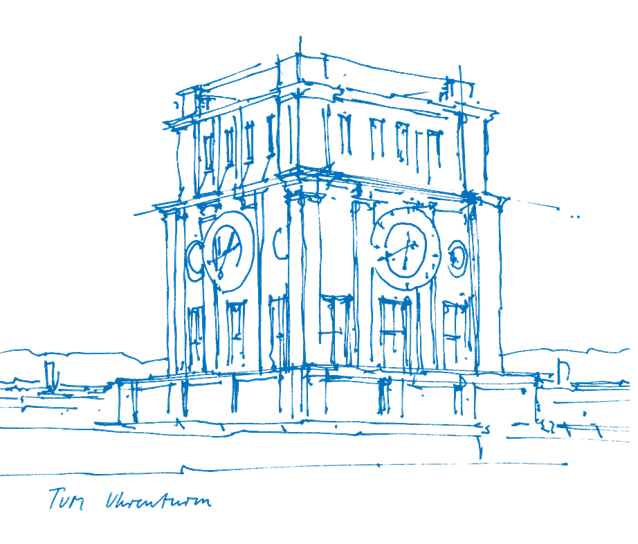
\includegraphics[width=0.65\textwidth]{TUM_Uhrenturm}
    \caption{Definition of the nodes and edges of a face and orientation of the local coordinate system}
    \label{fig:2Del}
  \end{center}
\end{figure}


%_________________________________________
\section{Tables}
\label{ssec:hosf_2D_sf}

Of course, you can use tables in your work as well; but please, do me the favor and consult Google. Remember: LaTeX is not about formating stuff. So, please do not spend time on how to format stuff; spend time writing!

\begin{table}
\caption{Size of the eigenvalue problem and time needed to achieve a mean error variance with a value of round $9.034\cdot10^{-2}$;
two-dimensional example of a plate with a hole; $M=8$}
  \begin{tabular*}{\textwidth}{@{\extracolsep{\fill}} l r  r l }
    \hline
    Method & $N$ & time & RF info \\
    \hline
    EOLE 				& 1040 		& $0.10s$ 	& 81 points per $m^2$\\
    FC-KL ($N_{el}=1$, tensor space) 	& 49 		& $1.7s$ 	& $p_{max}=6$ \\
    FC-KL ($N_{el}=1$, trunk space) 	& 47 		& $2.1s$ 	& $p_{max}=8$ \\
    FC-KL ($N_{el}=4$, tensor space) 	& 81 		& $3.7s$ 	& $p_{max}=4$ \\
    FC-KL ($N_{el}=4$, trunk space) 	& 69 		& $4.5s$ 	& $p_{max}=5$ \\
    FC-KL ($N_{el}=16$, tensor space) 	& 169 		& $15.4s$ 	& $p_{max}=3$ \\
    FC-KL ($N_{el}=16$, trunk space) 	& 105 		& $14.2s$ 	& $p_{max}=3$ \\
    \hline
  \end{tabular*}
\label{tab:2dex_2dhole_meanvar_m8_time1}
\end{table}


\section{Unterkapitelüberschrift}
\subsection[]{Absatzüberschrift}

Dies ist die Vorlage für eine wissenschaftliche Arbeit nach dem Corporate Design der Technischen Universität München (TUM). Die Vorlage ist für "`TeX Live 2015"' kompatibel.

Bitte geben Sie Ihren individuellen Text an den vorgesehenen Stellen ein und beachten Sie die Formatvorgaben des jeweiligen Lehrstuhls oder der Prüfenden zum inhaltlichen und formalen Aufbau der wissenschaftlichen Arbeit. Achten Sie grundsätzlich auf ein angenehmes Erscheinungsbild für den Leser und dass ein 1,5-facher Zeilenabstand und am Rand genügend Platz für Korrekturen eingehalten wird\footnote{Bitte beachten Sie die Zitationsvorgaben Ihres Prüfers.}.

Grundsätzlich sind die Schriftarten Arial und Times New Roman, sowie die Neue Helvetica zulässig. Der Text ist links ausgerichtet und in Blocksatz gesetzt. Auszeichnungen der Schrift können durch Fettung, Schrägstellung und Unterstreichung erfolgen. Farbige Schrift sollte nur in Ausnahmefällen oder Grafiken zum Einsatz kommen.
\begin{figure}[!ht]
\noindent\hspace{0.5mm}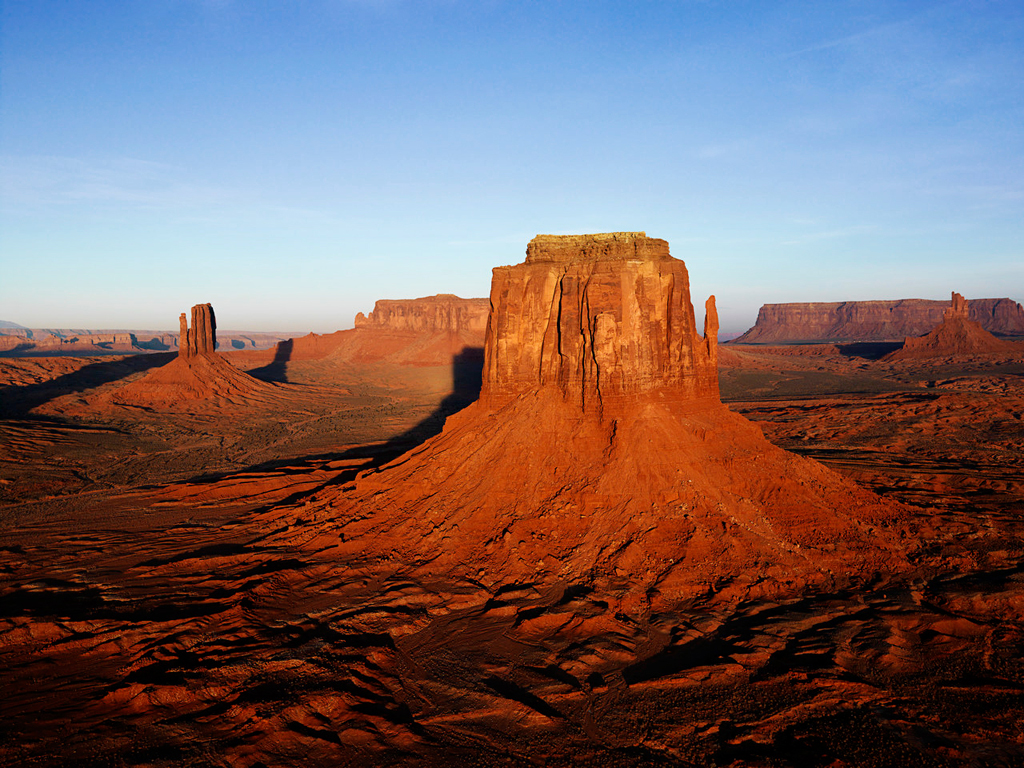
\includegraphics[width=12cm]{Desert.jpg}
\caption{Titel, Autor}
\end{figure}

Passen Sie gegebenenfalls die Ränder an die Vorgaben Ihres Prüfers an und beachten Sie dabei, dass das Logo der TUM sich oben rechts innerhalb der Ränder, auf der Titelseite befindet. Für die Titelseiten stehen separate
Vorlagen zur Verfügung.



\subsection[]{Aufzählungen}
\begin{itemize}
\item Dies ist die Standardaufzählung
    \begin{itemize}
    \item Dies ist die nächste Ebene der Aufzählung
    \end{itemize}
\end{itemize}


\subsection[]{Nummerierungen}
\begin{enumerate}
\item Erster Punkt der Nummerierungen
    \begin{enumerate}
    \item Unterpunkt der Nummerierungen
    \end{enumerate}
\end{enumerate}


% \addchap{Tabellenvarianten}
% 
% \vspace{22mm}
% \section*{Überschrift Tabelle 1}
% 
% \begin{table}[!h]
% \begin{tabularx}{\textwidth + 5pt}{@{\hspace{3pt}} M | @{\hspace{3pt}} M}
% \multicolumn{2}{@{}X}{%
%     \begin{tabularx}{\textwidth}{@{\hspace{3pt}} M @{\hspace{14.5pt}} M}
%     \textbf{Spalte 1} & \textbf{Spalte 2}
%     \end{tabularx}%
% } \\
% \hline
% Nummer 1 & Nummer 2 \\
% \hline
% Nummer 1 & Nummer 2 \\
% \hline
% Nummer 1 & Nummer 2 \\
% \hline
% \end{tabularx}
% 
% \caption{Beschreibung}
% \end{table}
% 
% 
% \vspace{\parskip}
% \section*{Überschrift Tabelle 2}
% 
% \begin{table}[!h]
% \hspace{-5pt}
% \begin{tabularx}{\textwidth + 5pt}{| @{\hspace{3pt}} M | @{\hspace{3pt}} M |}
% \hline
% \textbf{Spalte 1} & \textbf{Spalte 2} \\
% \hline
% Nummer 1 & Nummer 2 \\
% \hline
% Nummer 1 & Nummer 2 \\
% \hline
% Nummer 1 & Nummer 2 \\
% \hline
% \end{tabularx}
% \caption{}
% \end{table}
% 
% 
% \vspace{\parskip}
% \section*{Überschrift Tabelle 3}
% 
% \begin{table}[!h]
% \begin{tabularx}{\textwidth}{@{} M M}
% \textbf{Spalte 1} & \textbf{Spalte 2} \\
% Nummer 1 & Nummer 2 \\
% Nummer 1 & Nummer 2 \\
% Nummer 1 & Nummer 2 \\
% \end{tabularx}
% \caption{}
% \end{table}
% 
% 
% 
% \section{Tabellenvarianten 2}
% 
% \vspace{22mm}
% \section*{Überschrift Tabelle 1}
% 
% \begin{table}[!h]
% \fontsize{9pt}{13pt}\selectfont
% %\renewcommand{\arraystretch}{1.8}
% \hspace{-5pt}
% \begin{tabularx}{\textwidth + 5pt}{@{\hspace{3pt}} M | @{\hspace{3pt}} M}
% \multicolumn{2}{@{}X}{%
%     \begin{tabularx}{\textwidth}{@{\hspace{3pt}} M @{\hspace{14.5pt}} M}
%     \textbf{Spalte 1} & \textbf{Spalte 2}
%     \end{tabularx}%
% } \\
% \hline
% Nummer 1,\newline\,mehrzeilig in Schriftgröße 9 pt & Nummer 2 \\
% \hline
% Nummer 1 & Nummer 2 \\
% \hline
% Nummer 1 & Nummer 2 \\
% \hline
% \end{tabularx}
% 
% \caption{}
% \end{table}


% \vspace{\parskip}
% \section*{Überschrift Tabelle 2}
% 
% \begin{table}[!h]
% \fontsize{9pt}{13pt}\selectfont
% \hspace{-5pt}
% %\renewcommand{\arraystretch}{1.8}
% \begin{tabularx}{\textwidth + 5pt}{| @{\hspace{3pt}} M | @{\hspace{3pt}} M |}
% \hline
% \textbf{Spalte 1} & \textbf{Spalte 2} \\
% \hline
% Nummer 1 & Nummer 2 \\
% \hline
% Nummer 1 & Nummer 2 \\
% \hline
% Nummer 1 & Nummer 2 \\
% \hline
% \end{tabularx}
% \caption{}
% \end{table}
% 
% 
% \vspace{\parskip}
% \section*{Überschrift Tabelle 3}
% 
% \begin{table}[!h]
% \fontsize{9pt}{13pt}\selectfont
% %\renewcommand{\arraystretch}{1.8}
% \begin{tabularx}{\textwidth}{@{} M M}
% \textbf{Spalte 1} & \textbf{Spalte 2} \\
% Nummer 1 & Nummer 2 \\
% Nummer 1 & Nummer 2 \\
% Nummer 1 & Nummer 2 \\
% \end{tabularx}
% \caption{}
% \end{table}

%---------- References ----------
\cleardoublepage
\addcontentsline{toc}{chapter}{Bibliography}
\printbibliography
%
\cleardoublepage
\addcontentsline{toc}{chapter}{Index}
\printindex

\end{document}